Negli ultimi anni, un numero sempre crescente di infrastrutture critiche è stato digitalizzato, aggiungendo capacità di comunicazione e di computazione a numerosi dispositivi nelle reti di distribuzione dell'energia e dell'acqua, sistemi di trasporto, e manifatturieri. Ciò avviene in parte con lo scopo di aumentare l'efficienza, ma spesso è anche un requisito necessario a gestire l'ambiente che muta, come ad esempio la generazione locale dell'energia o il passaggio ai veicoli elettrici nel caso della distribuzione energetica.\\
Un progetto di digitalizzazione molto visibile è il passaggio dai \emph{meter} analogici ai digitali (\emph{smart}), che è attualmente in corso in vari paesi del mondo. Oltre ad una fatturazione complessivamente più precisa, uno smart meter può anche dare input agli algoritmi di controllo della grid, essere usato nei mercati energetici, comunicare con la \emph{smart home} (ad esempio, per regolare l'aria condizionata ed i sistemi di riscaldamento quando la richiesta energetica è alta), oppure per disconnettere da remoto un consumatore. In questo modo, un dispositivo precedentemente disconnesso e non critico si trasforma in un dispositivo connesso che può generare dati \emph{process-critical}.\\
La robustezza dei dati e dei comandi di switch è vitale - se una grande quantità di famiglie viene disconnessa simultaneamente, l'energia in eccesso non ha dove andare, potrebbe danneggiare la grid. In maniera simile, se gli algoritmi di manutenzione si basano su dati provenienti da misure effettuate dagli smart meter, input errati possono produrre effetti di gran lunga peggiori delle frodi di fatturazione. Ciò pone una nuova sfida per i produttori di meter: progettare dispositivi economici, largamente distribuiti e che lavorino su canali con banda banda molto ristretta.
\section{Open Smart Grid Protocol}
L'Open Smart Grid Protocol (OSGP) è stato uno dei primi protocolli di comunicazione su powerline per smart meters disponibile sul mercato, ed è largamente utilizzato per comunicare tra smart meter e l'aggregatore di dati, il quale è un dispositivo che colleziona dati provenienti da diverse centinaia di meter in un segmento di PLC (Power Line Communication) e li inoltra ad un controllore centralizzato.\\
L'OSGP risiede nel layer delle applicazioni dello stack protocollare definito dallo standard 14908 ISO/IEC \cite{standard14908}. Nonostante l'OSGP sia principalmente utilizzato per applicazioni di smart-metering, esso è stato progettato per un utilizzato più ampio all'interno di dispositivi della Smart Grid. Lo stack protocollare è molto leggero. Tale leggerezza è ottenuta pagando in sicurezza, infatti le primitive crittografiche consigliate dal NIST  (ad esempio: Advanced Encryption Standard - AES, in \emph{authenticated mode}) sono evitate, optando per altre meno intense computazionalmente: lo stream cipher RC4 per la cifratura ed una funzione digest non standard per l'autenticazione dei messaggi.\\
Il problema più grande è la combinazione di uno stream cipher con una funzione di digest lineare, che apre le possibilità per attacchi alle chiavi crittografiche ed ai messaggi. Ad esempio, si potrebbe sfruttare tale vulnerabilità utilizzando il ricevente di un messaggio come un ``oracolo". Dato un messaggio propriamente cifrato ed autenticato, un attaccante ipotizza una combinazione di un bit del messaggio ed un bit della chiave, invia un messaggio al ricevente appositamente confezionato, ed utilizza la risposta del  dispositivo che rifiuti o confermi l'ipotesi. Siccome questo può essere effettuato per singoli bit, un attaccante può ricostruire la chiave principale del dispositivo (OMA key) con al più $96 \times 3$ risposte.
\subsection{Potenziali debolezze del protocollo}
Sono state identificate quattro potenziali debolezze nel protocollo OSG.
\subsubsection{Utilizzo di RC4}
Negli ultimi anni sono state identificate varie debolezze nello stream cipher RC4. Uno dei problemi è la correlazione tra la chiave ed il \emph{keystream} di RC4 che può essere utilizzata per ricostruire la chiave. Questa debolezza è stata sfruttata con successo attraverso i vettori di inizializzazione (IVs)  utilizzati per ``rompere" WEP (Wired Equivalent Protection), standard che fa largo uso di RC4. Gli attacchi \cite{wep1}, \cite{wep2} rompono WEP in pochi secondi e tool per l'attacco come Aircrack-ng \cite{aircrackng} sono disponibili gratuitamente per effettuare penetration testing \cite{kali}.\\
L'uso di RC4 nel protocollo OSG è simile al modo in cui RC4 era usato nello standard WEP. Mentre, per ogni messaggio, è generata una nuova chiave, solamente i primi 8 byte della chiave variano, ed i restanti 8 byte sono costanti. Inoltre, gli 8 byte iniziali vengono messi in XOR con un valore noto pubblicamente. Sebbene gli autori non siano a conoscenza di un attacco reale a tale caratteristica, ciò implica una forte correlazione tra le chiavi usate, e fornisce ad un attaccante dati interessanti da analizzare. Ulteriormente, l'impostazione è simile a quella utilizzata nello standard WEP, questo lascia intuire che c'è una grande esperienza nel campo dello \emph{statistical key recovery}.\\
Un altro problema di RC4 in OSGP è che è utilizzato con una autenticazione debole. Data la natura di uno stream cipher, un attaccante che entra in possesso di un \emph{ciphertext} può alterare bit in posizioni scelte. Grazie alla conoscenza dello spazio dei messaggi dello standard EN 14908, un attaccante può inviare messaggi alterati che sono validi con alta probabilità. Inoltre, egli può autenticare questo messaggi sfruttando la debolezza della funzione di digest descritta qui di seguito.
\subsubsection{Debole funzione di digest}
La funzione di digest utilizzata nel protocollo OSG per l'autenticazione dei messaggi è lineare ed è implementata in un modo che non solo disabilita l'autenticazione ma può inoltre decifrare un messaggio intercettato in tempo lineare nella lunghezza del messaggio. La debolezza strutturale intrinseca alla funzione di digest consente un attacco ``man-in-the-middle" (che dimezza la taglia della chiave per un attacco di forza bruta), la modifica dei messaggi in maniera controllata, ricomputazione del digest corretto senza il bisogno di cifratura - o di chiavi di autenticazione, ed utilizzando i messaggi di NACK di un dispositivo su un digest errato per ricostruire sia la chiave di autenticazione che il messaggio.
\subsubsection{Sicurezza di broadcast non definita}
Nonostante la funzione di broadcast sia chiamata ``Secure Broadcast", la sicurezza definita su di essa è molto bassa. Questo è particolarmente preoccupante, se si pensa che tale meccanismo è utilizzato per inviare aggiornamenti del firmware, che sono distribuiti attraverso il meccanismo di broadcast sicuro senza alcuna misura specifica atta a fornire autenticazione dalla sorgente.
\subsubsection{Utilizzo della chiave}
Sebbene il protocollo faccia uso di chiavi di sessione per la cifratura, utilizza una master key per l'autenticazione. Comunque, questa chiave di autenticazione è usata per derivare la cifratura delle chiavi di sessione. Quindi se la chiave di autenticazione è compromessa, tutte le chiavi di sessione sono note dall'attaccante. Siccome la chiave di autenticazione è usata con un debole algoritmo di autenticazione, essa è altamente esposta ad un gran numero di attacchi, e comprometterla è ben possibile.
\subsection{Sfruttare le debolezze strutturali}
Queste debolezze strutturali possono essere sfruttate in vari modi. Gli attacchi adatti a tale scopo complessivamente non sono molto sofisticati, piuttosto, grazie alla debolezza dei \emph{building block} crittografici un attaccante è capace di dirottare un intero segmento PLC.\\
Un attacco relativamente semplice punta a \textit{rompere} la funzione di digest così che un attaccante possa non solo forgiare messaggi, ma - avendo ottenuto accesso ad un messaggio autentico di sufficiente lunghezza - anche ricostruire chiavi crittografiche con basso sforzo, per poi inviare falsi comandi correttamente autenticati.
%-----------------------------------------------------------------------------
%\section{Attacchi}
\section{Attacking Smart Meters and Smart Devices}
Uno dei maggiori argomenti utilizzati per mettere in sicurezza gli smart meter è che i consumatori avranno accesso fisico, e potenzialmente anche logico, a tali dispositivi. Sebbene i consumatori avessero accesso ai vecchi meter, questi ultimi non operavano utilizzando tecnologie familiari ai consumatori o a cui potessero avere accesso. A causa della prevalenza di queste tecnologie ben note, gli smart meter possono essere trattati come obiettivi tradizionali, quando ci si trova ad applicare metodologie di \emph{security testing} su di essi.\\
Di seguito vengono analizzate due tra le più comuni metodologie di security testing e come queste possano essere applicate al testing degli smart meter.

\subsection{Open Source Security Testing Methodology Manual}
Nel Gennaio 2001 , in USA e Spagna, fu fondato l'Institute for Security and Open Methodologies (ISECOM): organizzazione no-profit il cui scopo è quello di fornire soluzioni pratiche per security awareness, ricerca, certificazione e business integrity. Il loro \emph{Open Source Security Testing Methodology Manual} (OSSTMM) fornisce agli utenti le metodologie per effettuare security testing. L'OSSTMM contiene sei sezioni che recensiscono un numero enorme di aspetti di sicurezza, incluse reti, dispositivi wireless, e sicurezza fisica. Per tali aspetti, è possibile applicare l'OSSTMM al security testing degli smart meter.\\
Sezioni dell'ISECOM \emph{Open Source Security Testing Methodology Manual}:
\begin{enumerate}
	\item Information Security
	\item Process Security
	\item Internet Technology Security
	\item Communications Security
	\item Wireless Security
	\item Physical Security
\end{enumerate}
Eseguire security testing in accordo all'OSSTMM richiede che ogni modulo contenuto in ogni sezione sia testato ed elenca sei approcci comuni al testing: dal Double Blind, in cui sia target che attaccante non abbiano informazioni prima di condurre il testing, al Tandem, dove il target e l'attaccante condividono informazioni riguardo il testing apertamente. L'approccio mostrato di seguito è quello Double Blind in quanto è quello che più si avvicina ad una situazione reale.
\subsubsection{Information Security}
In questa sezione risiedono otto moduli:
\begin{enumerate}
	\item Posture assessment
	\item Information integrity review
	\item Intelligence survey
	\item Internet document grinding
	\item Human resources review
	\item Competitive intelligence review
	\item Privacy controls review
	Information controls review
\end{enumerate}
La sezione di Information Security dell'OSSTMM si concentra su \emph{information gathering} e \emph{validation}. Dalla prospettiva di un attaccante, include l'ottenimento e la revisione di informazioni riguardo la marca e modello dello smart meter target per studiarne il funzionamento, gli standard utilizzati e determinare quali attacchi possano essere più adatti rispetto ad altri.


\subsubsection{Process Security Testing}
La seconda sezione dell'ISECOM \emph{Open Source Security Testing Methodology Manual} si concentra sull'analisi di sicurezza dei processi del target e contiene i seguenti cinque moduli:
\begin{enumerate}
	\item Posture review
	\item Request testing
	\item Reverse Request testing
	\item Guided Suggestion testing
	\item Trusted Persons testing
\end{enumerate}

La seconda sezione, quindi, si occupa di ciò che solitamente è chiamata ``social engineering". Ogni modulo punta ad ottenere informazioni da persone attraverso la coercizione e l'inganno. In relazione ad attaccare gli smart meter, ciò include impersonare il tecnico di una compagnia o un consumatore.\\
Con questi metodi, sarebbe possibile ottenere informazioni di valore come specifiche tecniche o amministrative, o credenziali degli utenti.

\subsubsection{Internet Technology Security Testing}
La maggior parte dei moduli applicabili al testing della sicurezza degli smart meter è contenuta nei quattordici moduli di questa sezione:
\begin{enumerate}
	\item Network Surveying
	\item Port Scanning
	\item Services Identification
	\item System Identification
	\item Vulnerability Research and Verification
	\item Internet Application Testing
	\item Router Testing
	\item Trusted Systems Testing
	\item Firewall Testing
	\item Intrusion Detection System Testing
	\item Containment Measures Testing
	\item Password Cracking
	\item Denial of Service Testing
	\item Security Policy Review
\end{enumerate}

\paragraph{Network Surveying}\mbox{}\\
Punta all'identificazione dei sistemi target accessibili in rete. Nel caso di smart meters, questi sono accessibili agli attaccanti attraverso sia reti wireless che le home area networks. In entrambi i casi, il Network Surveying consiste nell'ottenere informazioni sui target (\emph{information gathering}). 
Ciò può essere realizzato in uno dei seguenti modi: passivamente, ascoltando il traffico di passaggio sulla rete, o attivamente, facendo \emph{IP probing} in attesa di una response.\\

\begin{figure}[hbtp]
	\centering
	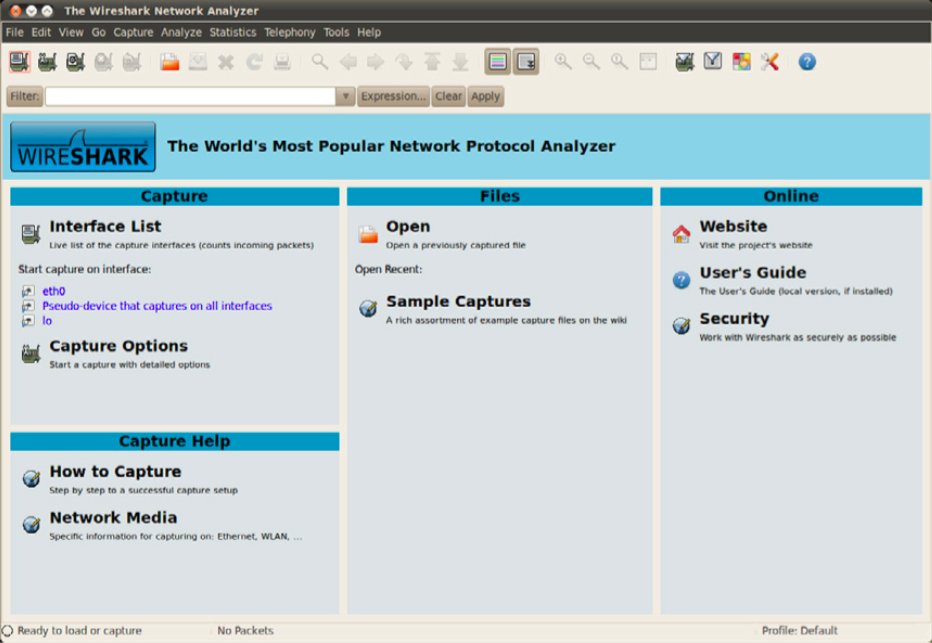
\includegraphics[scale=.3]{imgs/attack/wireshark.png}
	\caption{Wireshark sniffing tool}
	\label{wireshark_img}
\end{figure}

Per l'identificazione passiva, può essere utilizzato Wireshark fig. \ref{wireshark_img}.\cite{wireshark} Wireshark cattura il traffico che attraversa qualsiasi rete in tempo reale e fornisce l'ispezione di centinaia di protocolli. È possibile inoltre specificare gli indirizzi IP di cui effettuare lo sniffing, così da limitare la raccolta di informazione ai possibili target.\\
Per quanto riguarda l'identificazione attiva, invece, è possibile utilizzare la tecnica del \emph{ping sweep}: essa si avvale del Internet Control Message Protocol (ICMP) per individuare i target attivi in rete analizzando le loro response. Nel caso in cui il traffico ICMP sia bloccato, è spesso utilizzato il ping di TCP. Per entrambi i casi è utilizzato il tool di sicurezza Nmap.\cite{nmap}

\paragraph{Port Scanning}\mbox{}\\
Consiste nel fare \emph{probing} sul target in attesa di risposte sulle 65,536 porte TCP e/o UDP. Ottenere una response significa che dei servizi sono in esecuzione sulle porte associate e che potrebbero contenere debolezze che esporrebbero il target. Il tool di port-scanning più utilizzato è Nmap, che permette di effettuare scan TCP completando l'\emph{handshake}, o attraverso scan TCP SYN che utilizza solamente i messaggi iniziali di SYN e SYN ACK dell'\emph{handshake} TCP.\\
L'OSSTMM suggerisce che la scelta di quali delle 65,536 porte da analizzare è a discrezione dell'attaccante e dipende dal contesto.

\paragraph{Services Identification and System Identification}\mbox{}\\
Lo scopo di questi due moduli è di enumerare i servizi in esecuzione sulle porte TCP o UDP che hanno prodotto una response nella fase di port scanning, così come identificare il sistema operativo del target.\\
Entrambi i compiti sono svolti dal tool Nmap, attivando lo switch \textbf{-sV} che fornisce informazioni addizionali ad esempio il numero di versione, come è possibile verificare nella fig. \ref{nmap_sv_img}.\\
In questo caso il target utilizzato, \emph{webserver.domain.com}, fornisce informazioni quali il sistema operativo in quanto esposte dal server web Apache. Un attaccante userebbe le informazioni ottenute per verificare la presenza di falle nelle specifiche versioni dei servizi, per poi preparare un attacco.
\begin{figure}[hbtp]
	\centering
	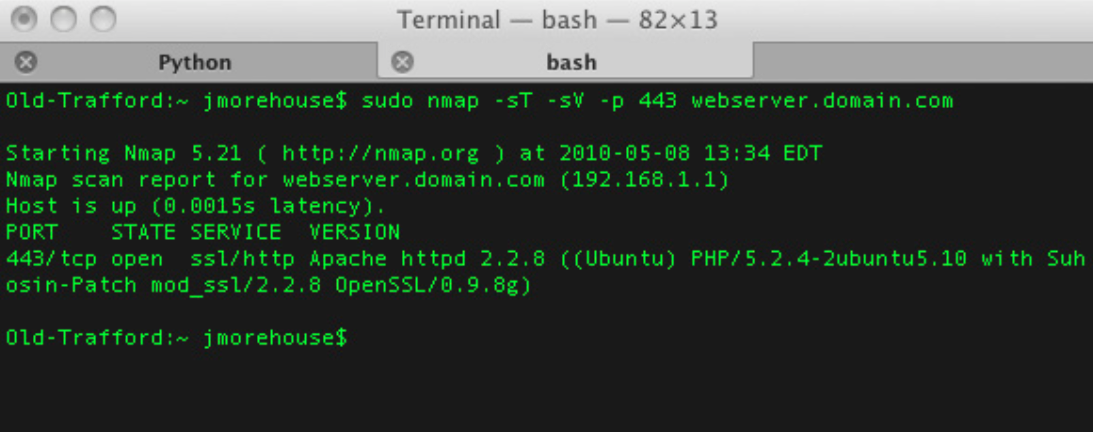
\includegraphics[scale=.3]{imgs/attack/nmap_sv.png}
	\caption{Nmap version detection ouput}
	\label{nmap_sv_img}
\end{figure}

\paragraph{Vulnerability Research and Verification}\mbox{}\\
Una volta noti sistema operativo e servizi in esecuzione con relative versioni si passa alla ricerca  e verifica di vulnerabilità tramite testing manuale ed automatizzato.\\
Un tool comunemente utilizzato per effettuare tale scan è Nessus \cite{nessus}, sviluppato dalla Tenable Network Security mostrato in fig. \ref{nessus_img}. Sebbene Nessus sia ottimo per eseguire scanning automatizzato per determinare debolezze come una versione non aggiornata di Apache, il testing manuale dovrebbe coadiuvare quello automatizzato per individuare debolezze che potenzialmente potrebbero essere trascurate.\\
\begin{figure}[hbtp]
	\centering
	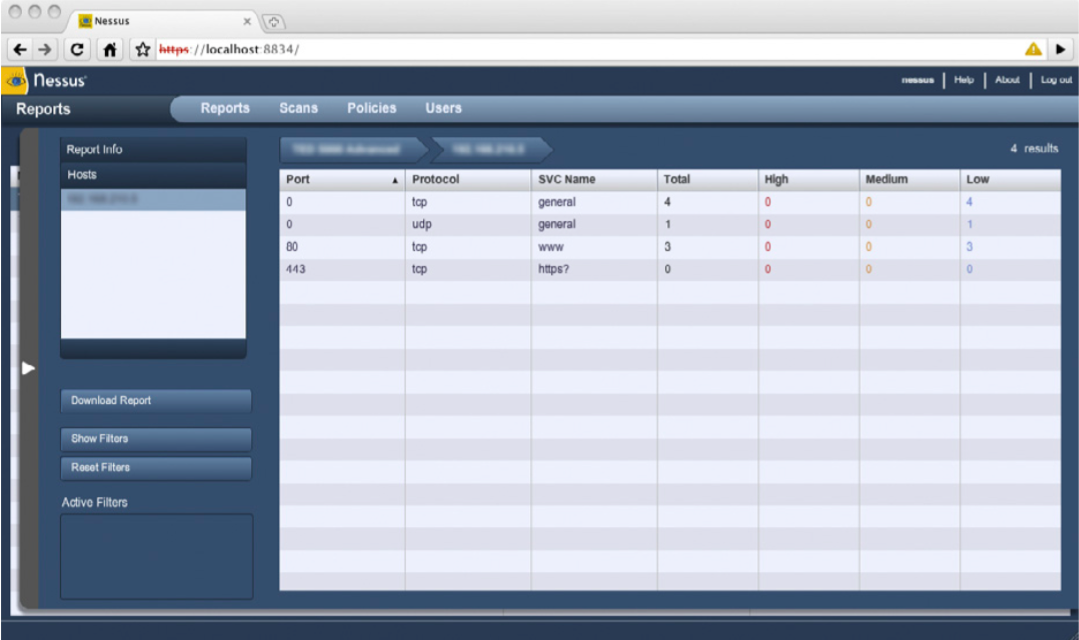
\includegraphics[scale=.3]{imgs/attack/nessus.png}
	\caption{Interfaccia web di Nessus}
	\label{nessus_img}
\end{figure}
L'OSSTMM consiglia che il testing automatizzato venga effettuato da almeno due scanner seguito da una verifica manuale. Le tecniche utilizzate per la verifica manuale di vulnerabilità variano molto in funzione della vulnerabilità che si sta cercando, come ad esempio l'uso di Telnet per osservare la versione di uno specifico servizio connettendocisi, o l'utilizzo di un client FTP per connettersi ad un server FTP anonimo.\\
Nel processo di attacco a smart meter, la fase in esame è un passo critico in quanto fornisce i potenziali punti d'ingresso nello smart meter che potrebbero essere sfruttati nel modulo che segue.

\paragraph{Internet Application Testing}\mbox{}\\
Spesso, gli scanner di vulnerabilità non includono la possibilità di eseguire identificazione di vulnerabilità e verifica per Web application.\\
Con l'aumentare delle misure di sicurezza adottate dai produttori di sistemi all'interno del proprio ciclo di sviluppo, il numero di servizi in esecuzione a disposizione di attaccanti si è man mano ridotto. Ciò ha portato questi ultimi a concentrarsi sulle web application in esecuzione sui dispositivi target. Nel caso degli smart meter, tali applicazioni consentono al consumatore di visualizzare o configurare le informazioni di utilizzo, o permettono ai tecnici di configurare il dispositivo. Lo scopo di questo modulo è lo stesso del precedente, ma in un ambiente differente.\\
Effettuare identificazione e verifica di vulnerabilità su web application è significativamente più complesso che eseguire lo stesso test su servizi in esecuzione. Questo è il risultato del livello di personalizzazione trovato in ogni web application: è raro il caso che una web application sia esattamente come un'altra, ed anche nel caso di due \emph{webapp} identiche trovate in esecuzione, la loro infrastruttura di backend potrebbe differire. Per questo il testing manuale gioca un ruolo significativo e i tool a supporto di tale operazione sono molteplici. L' Open Web Application Security Project (OWASP) ha sviluppato una guida al testing per le web application, disponibile a questo indirizzo \url{https://www.owasp.org/index.php/Category:OWASP_Testing_Project}.

\paragraph{Password Cracking}\mbox{}\\
Questo modulo consiste nell'individuazione delle credenziali valide di un servizio in esecuzione o di una web application. Il testing può essere effettuato sia a partire da una lista precompilata di password, noto come attacco basato su dizionario, che provando ogni possibile combinazione di un certo alfabeto di caratteri, noto come attacco brute force.\\
Quando si esegue password cracking, è bene tenere a mente che molti servizi e web application implementano un servizio di blocco temporaneo o permanente, che disabilita un account se si verificano troppi tentativi di accesso con password invalide durante un determinato periodo di tempo.\\
Un tool comunemente utilizzato nell'ambito del password cracking, che supporti sia attacchi con dizionario che brute force, è Cain & Abel \cite{cainabel}, mostrato in fig. \ref{cainabel_img}.\\
\begin{figure}[hbtp]
	\centering
	\includegraphics[scale=.3]{imgs/attack/cainable.png}
	\caption{Il tool di password cracking Cain & Abel}
	\label{cainable_img}
\end{figure}
Il password cracking ha un ruolo fondamentale nell'attacco ad uno smart meter quando ci si trova davanti ad un prompt di autenticazione. Se un attaccante riesce ad ottenere le credenziali di uno smart meter, egli può istantaneamente avere accesso al dispositivo.

\paragraph{Denial of Service Testing}\mbox{}\\
Il modulo di Denial of Service si occupa di identificare i punti deboli che potrebbero essere del device stesso o all'interno dell'infrastruttura sottostante. Tale operazione potrebbe coinvolgere l'utilizzo degli strumenti precedentemente descritti, Wireshark e Nmap. Ad esempio, Wireshark potrebbe essere utilizzato per determinare i regolari pattern di traffico da e verso lo smart meter. Nmap invece potrebbe essere utilizzato per incrementare gradualmente il traffico verso lo smart meter nell'intento di sovraccaricare il dispositivo o la sua infrastruttura.\\
Se l'obiettivo dell'attaccante è semplicemente di negare il servizio ad uno smart meter, sarebbe molto semplice condurre un attacco del genere se comparato con attacchi che mirano alla compromissione della confidenzialità e/o integrità dello smart meter.

\paragraph{Exploit Testing}\mbox{}\\
Tutti i moduli descritti fin'ora gettano le basi per l'esecuzione dell'exploit testing. L'exploit testing punta ad utilizzare le vulnerabilità identificate per compromettere lo smart meter. Esempio di exploit testing includono l'utilizzo di codice per sfruttare un buffer overflow in un servizio in esecuzione o utilizzando SQL injection per accedere ad una shell di comando attraverso una falla nella validazione di un input all'interno di una web application.\\
Metasploit è un exploit tool disponibile gratuitamente che offre ai tester di sicurezza e agli attaccanti un considerevole numero di \emph{vulnerability exploit} e \emph{payload}. \cite{metasploit}
\begin{figure}[hbtp]
	\centering
	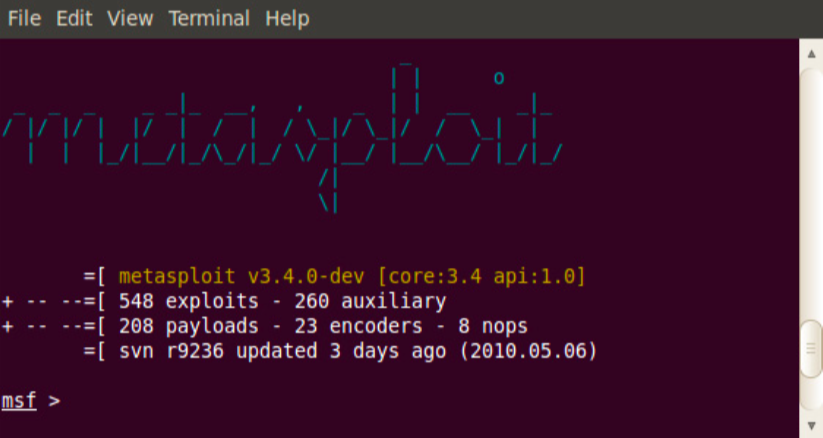
\includegraphics[scale=.3]{imgs/attack/metasploit.png}
	\caption{Il tool di vulnerability exploit Metasploit}
	\label{metasploit_img}
\end{figure}
Per un security tester, lo scopo finale è spesso quello di compromettere il target, laddove per un attaccante, la sola compromissione dello smart meter possa essere un altro passo nella propria metodologia personale di raggiungere l'obiettivo preposto.
\section{False Data Injection}
\section{Time Delay Attack}
\section{Replay Attack}
\section{Jamming}
\section{Web Application}
\section{Rilevamento}
\section{Power Fingerprinting}
\section{Optimal Malicious Attack Construction and Robust Detection in Smart Grid Cyber Security Analysis}



\begin{thebibliography}{99}
\bibitem{standard14908} International Organization for Standardization. ISO/IEC 14908-1:2012:Information technology – Control network protocol – Part 1: Protocol stack, 2012.
\bibitem{wep1} Andreas Klein. \emph{Attacks on the RC4 stream cipher.} Des. Codes Cryptography, 48(3):269–286, 2008.
\bibitem{wep2} Erik Tews, Ralf-Philipp Weinmann, and Andrei Pyshkin. \emph{Breaking 104 bit WEP in less than 60 seconds.} In Sehun Kim, Moti Yung, and Hyung-Woo Lee, editors, Information Security Applications, 8th International Workshop, WISA 2007, Jeju Island, Korea, August 27-29, 2007, Revised Selected Papers, volume 4867 of Lecture Notes in Computer Science, pages 188–202. Springer, 2007.
\bibitem{aircrackng} Aircrack-ng. \url{http://www.aircrack-ng.org/}
\bibitem{kali} Kali Linux. \url{https://www.kali.org/}
\bibitem{wireshark} Wireshark. \url{https://www.wireshark.org/}
\bibitem{nmap} Nmap. \url{https://www.nmap.org/}
\bibitem{nessus} Nessus. \url{https://www.nessus.org/}
\bibitem{cainabel} Cain & Abel. \url{http://www.oxid.it/}
\bibitem{metasploit} Metasploit. \url{http://www.metasploit.com/}
\end{thebibliography}